% % % % % % % % % % % % % % % % % % % % % % % % % % % % % % % %
\begin{frame}
\frametitle{Midpoint Approximation}
Taking $x_i^*$ to be the midpoint $\bar x_i=(x_{i-1}+x_i)/2$, we get the
{\bf Midpoint Approximation}.  $ M_n $ is typically a better approximation than either $ L_n $ or $ R_n$.
\[
\int_a^b f(x)dx \approx M_n = \Delta x\big[f(\bar x_1)+\dots + f(\bar
x_n)\big].
\]
\[
\Delta x=\frac{b-a}{n}
\]

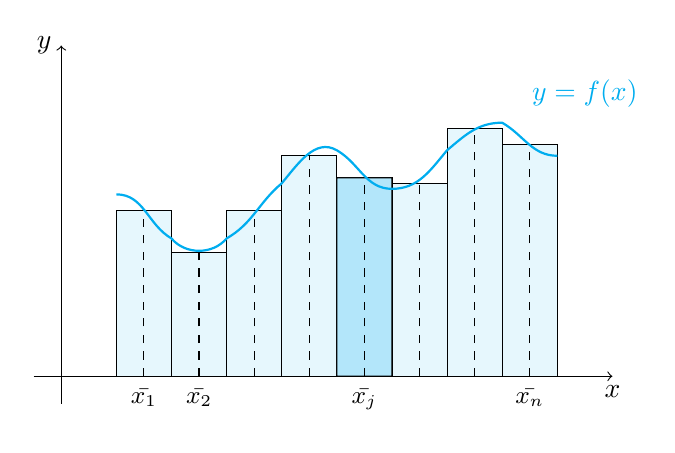
\begin{tikzpicture}[scale=.7]


\coordinate (p1) at (0.7,3);
\coordinate (p2) at (1,3.3);
\coordinate (p3) at (2,2.5);
\coordinate (p4) at (3,2.5);
\coordinate (p5) at (4,3.5);
\coordinate (p6) at (5,4.1);
\coordinate (p7) at (6,3.4);
\coordinate (p8) at (7,4.1);
\coordinate (p9) at (8,4.6);
\coordinate (p10) at (9,4);
\coordinate (p11) at (9.5,4.7);

% The cyan background
%\fill[cyan!10] 
%  (p2|-0,0) -- (p2) -- (p3) -- (p4) -- (p5) -- (p6) -- (p7) -- (p8) -- (p9) -- (p10) -- (p10|-0,0) -- cycle;

 
% the broken line connecting points on the curve
 \draw[fill=cyan!10] (1,0) --(1,3)--(2,3)--(2,0)--(2,2.25)--(3,2.25)--(3,0)--(3,3)--(4,3)--(4,0)--(4,4)--(5,4)--(5,0)--(5,3.6)--(6,3.6)--(6,0)--(6,3.5)--(7,3.5)--(7,0)--(7,4.5)--(8,4.5)--(8,0)--(8,4.2)--(9,4.2) --(9,0) -- cycle;
% the dark cyan stripe
 \fill[cyan!30, draw= black] (p6|-0,0) -- (5,3.6) -- (6,3.6) -- (p7|-0,0) -- cycle;
% vertical lines and labels
\draw[dashed] (1.5,0) -- (1.5,3);
\node[below,text height=1.5ex,text depth=1ex,font=\small] at (1.5,0) {$\bar{x_1}$};
\draw[dashed] (2.5,0) -- (2.5,2.25);
\node[below,text height=1.5ex,text depth=1ex,font=\small] at (2.5,0) {$\bar{x_2}$};
\draw[dashed] (3.5,0) -- (3.5,3);
\node[below,text height=1.5ex,text depth=1ex,font=\small] at (3.5,0) { };
\draw[dashed] (4.5,0) -- (4.5,4);
\node[below,text height=1.5ex,text depth=1ex,font=\small] at (4.5,0) { };
\draw[dashed] (5.5,0) -- (5.5,3.6);
\node[below,text height=1.5ex,text depth=1ex,font=\small] at (5.5,0) {$\bar{x_j}$};
\draw[dashed] (6.5,0) -- (6.5,3.5);
\node[below,text height=1.5ex,text depth=1ex,font=\small] at (6.5,0) { };
\draw[dashed] (7.5,0) -- (7.5,4.5);
\node[below,text height=1.5ex,text depth=1ex,font=\small] at (7.5,0) { };
\draw[dashed] (8.5,0) -- (8.5,4.2);
\node[below,text height=1.5ex,text depth=1ex,font=\small] at (8.5,0) {$\bar{x_n}$};

% the curve
\draw[thick,cyan] 
   %(p1) to[out=70,in=180] 
   (p2) to[out=0,in=150] 
   (p3) to[out=-50,in=230] (p4) to[out=30,in=220] 
   (p5) to[out=50,in=150] (p6) to[out=-30,in=180] 
   (p7) to[out=0,in=230] (p8) to[out=40,in=180] 
   (p9) to[out=-30,in=180] (p10); 
   % to[out=0,in=260] (p11);
% The axes
\draw[->] (-0.5,0) -- (10,0) coordinate (x axis);
\draw[->] (0,-0.5) -- (0,6) coordinate (y axis);
% labels for the axes
\node[below] at (x axis) {$x$};
\node[left] at (y axis) {$y$};
% label for the function
\node[above,text=cyan] at (p11) {$y=f(x)$};

%\draw[help lines,step=.2] (-2,-2) grid (12,12);
\end{tikzpicture}
%\includegraphics[width=0.5\linewidth]{../../modules/approximate-integration/pictures/Left1}
%\includegraphics[width=0.5\linewidth]{../../modules/approximate-integration/pictures/Right1}


%\includegraphics[width=0.25\linewidth]{../../modules/approximate-integration/pictures/Left1}
%\includegraphics[width=0.5\linewidth]{../../modules/approximate-integration/pictures/MP1}
%\includegraphics[width=0.25\linewidth]{../../modules/approximate-integration/pictures/Right1}

\end{frame}
% % % % % % % % % % % % % % % % % % % % % % % % % % % % % % % %
